\documentclass[a4paper, 12pt]{article}
\usepackage[slovene]{babel}
\usepackage[utf8]{inputenc}
\usepackage{url}
\usepackage{hyperref}
\usepackage{listings}
\usepackage{amsmath}
\usepackage{amssymb}
\usepackage{float}
\usepackage{subcaption}
\usepackage{graphicx}
\graphicspath{ {C:/Users/dmoho/Documents/FRI/2_letnik_1_semester/VS/slike/} }

\begin{document}

\title{Najemnine v Ljubljani}
\author{Domen Mohorčič}
\maketitle

\section{Uvod}

Ko se povprečen Slovenec odseli od staršev v svoje stanovanje, je star 28,2
leti (\href{https://www.stat.si/statweb/News/Index/7570}{stat.si}). Pred
izselitvijo pa si mora stanovanje poiskati. Po navadi ljudje pri izbiri
stanovanja gledajo na to, ali jim je stanovanje všeč in ali se jim zdi cena
ustrezna stanovanju. Od česa pa sploh je odvisna cena stanovanja? Friškovec
(2010)[1] ugotavlja, da je oglaševalska cena stanovanja
pozitivno odvisna od površine, števila kopalnic in ali gre za mansardno
stanovanje, negativno pa predvsem od višine nadstropja. Repič (2014)[2] pa je
v magistrski nalogi pokazala, da je prodajna cena stanovanja pozitivno odvisna
od prisotnosti dvigala, parkirnega mesta, opremljenosti stanovanja, bližine
središča Ljubljane in števila sob v stanovanju, negativno pa na ceno vplivajo
starost stanovanja, površina in trajanje, ko je nepremičnina na voljo za
prodajo.

V Sloveniji v najemniških stanovanjih živi le 2,4
gospodinjstev (\href{https://cekin.si/nepremicnine/trnova-pot-do-lastnega-doma-zakaj-mora-biti-tako.html}{cekin.si}).
Kljub temu je trg najema nepremičnin kar velik, še posebej v Ljubljani (na
nepremicnine.net je od 1500 oglasov za najem, od tega kar 1000 v Ljubljani),
kjer pa so najbolj zaželjeni študentje ali posamezniki. Nikjer pa nisem
zasledil raziskave, ki bi ugotavljala, kaj vpliva na ceno najema.

Namen seminarske naloge je ugotoviti, kateri dejavniki najbolj vplivajo na ceno
najemnin v Ljubljanskima predeloma Vič in Rudnik.

\section{Podatki}

Podatke sem pridobil iz slovenske spletne strani
\href{https://www.nepremicnine.net}{nepremicnine.net} dne 8.8.2020.
Iskal sem stanovanja v Ljubljani v predelih Vič in Rudnik.
Pri pregledovanju oglasov sem se osredotočil na naslednje podatke:
nadstropje, v katerem se stanovanje nahaja, število vseh nadstropij v zgradbi,
leto gradnje stavbe, leto prenove stanovanja, število sob v stanovanju,
ali ima stanovanje shrambo/klet, ali je stanovanje opremljeno, število
pripadajočih parkirišč, velikost bivalne površine, zunanje površine
(balkon, vrt, \dots), mesečni stroški bivanja in cena najema. Ker pa sem hotel
ugotoviti, ali na ceno najema vpliva tudi lokacija stanovanja, sem poiskal še
oddaljenost do središča Ljubljane (v mojem primeru Prešernov trg). Na prej
omenjeni spletni strani pa v večini primerov ni napisanega točnega naslova,
zato sem iskal samo približne lokacije (ulica ali naselje).

Pri določanju razdalje sem si pomagal z orodjem
\href{https://www.distance.to/}{distance.to}. Za analizo podatkov sem uporabil
program \href{https://rstudio.com/}{RStudio}.

\subsection{Opis spremenljivk}

Zbrane podatke sem označil z naslednjimi spremenljivkami:
\begin{table}[h]
\begin{center}
\caption{Tabela spremenljivk in njihov opis}
\label{table:1}
\begin{tabular}{ c|c}
	spremenljivka & opis \\
	\hline
	\hline
	nadstropje & V katerem nadstropju se stanovanje nahaja \\
	\hline
	vsaNadstropja & Število vseh nadstropij v stavbi \\
	\hline
	letoGradnje & Leto, v katerem je bilo stanovanje zgrajeno \\
	\hline
	letoPrenove & Leto, v katerem je bilo stanovanje prenovljeno \\
	\hline
	stSob & Število sob v stanovanju \\
	\hline
	stParkirisc & Število parkirnih mest, ki pripadajo stanovanju \\
	\hline
	parkirisce & Ali stanovanju pripada lastno parkirišče \\
	\hline
	opremljenost & Kako je stanovanje opremljeno (polno, delno ali nič) \\
	\hline
	shramba & Ali stanovanju pripada zunanja soba za shranjevanje \\
	\hline
	zunanjePovrsine & Vsota zunanjih površin stanovanja \\
	\hline
	povrsina & Velikost bivalne površine v stanovanju \\
	\hline
	oddaljenost & Oddaljenost stanovanja od Prešernovega trga \\
	\hline
	cena & Cena mesečne najemnine stanovanja \\
	\hline
	stroski & Cena mesečnih stroškov bivanja \\
	\hline
	skCena & Seštevek cene in mesečnih stroškov bivanja \\
\end{tabular}
\end{center}
\end{table}

Za model napovedi mesečne najemnine sem izbral spremenljivke $ skCena $,
$ parkirisce $, $ povrsina $, $ letoGradnje $ in
$ oddaljenost $. $ skCena $ je odvisna spremenljivka, ostale štiri pa
so neodvisne.

Spremenljivko $ letoPrenove $ sem odstranil iz modela, ker za večino
stanovanj podatka nisem našel. $ nadstropje $ in $ vsaNadstropja $
sem izvzel, ker pri pregledu oglasov nisem dobil občutka, da bi ti dve
spremenljivki pomembno vplivali na ceno najemnine. Spremenljivko
$ opremljenost $ sem odstranil, ker je bilo $ 89.3\% $ stanovanj
opremljenih in tako ni bilo dovolj raznolikosti. Pri pregledu korelacijske
matrike sem ugotovil, da sta spremenljivki $ povrsina $ in
$ stSob $ povezani s korelacijskim koeficientom $ 0.811 $ zato sem obdržal
spremenljivko $ povrsina $. Namesto $ stParkirisc $ sem uporabil
spremenljivko $ parkirisce $, saj je tako bolje predstavljeno, ali ga
stanovanje ima. Spremenljivko $ zunanjePovrsine $ pa sem  odstranil iz
modela, ker je imela večina stanovanj samo balkon, redko pa so se pojavili
velikimi vrtovi.

\subsection{Analiza podatkov}

Izmed petih spremenljivk so $ letoGradnje $, $ povrsina $,
$ oddaljenost $ in $ skCena $ zvezne, $ parkirisce $ pa je
diskretna. Zbral sem podatke o 103 različnih stanovanjih ($ N = 103 $).

Za vsako zvezno spremenljivko sem izračunal povprečje, standardni odklon,
mediano absolutnih odstopanj od mediane, asimetričnost in sploščenost.
Povprečje se izračuna po formuli
\begin{equation}
	\mu = \frac{\sum\limits_{i=1}^{N} x_{i}}{N}
\end{equation}
Standardni odklon se izračuna po formuli
\begin{equation}
	\sigma = \sqrt{\frac{\sum\limits_{i=1}^{N}\left(x_{i}-\mu\right)^{2}}{N}}
\end{equation}
Mediano absolutnih odstopanj od mediane se izračuna tako, da se izračunajo vse
absolutne razlike med podatki in mediano in se poišče mediano razlik.
\newline
Asimetričnost se izračuna po naslednji formuli
\begin{equation}
	skew = \frac{\sum\limits_{i=1}^{N}\left(x_{i}-\mu\right)^{3}}{N*\sigma^{3}}
\end{equation}
Sploščenost pa se izračuna po formuli
\begin{equation}
	kurtosis = \frac{\sum\limits_{i=1}^{N}\left(x_{i}-\mu\right)^{4}}{N*\sigma^{4}}-3
\end{equation}

Asimetričnost (skewness) nam pove, kako asimetrični so podatki. Negativna
vrednost pove, da je rep podatkov na levi (večina podatkov je na desni stran
grafa) in obratno. Na grafu se to vidi kot v katero smer so podatki razvlečeni.
Vrednost $ 0 $ nam pove, da so podatki porazdeljeni simetrično, $ >0 $ pove, da
so podatki razvlečeni v desno, $ <0 $ pa da so razvlečeni v levo.

Sploščenost (kurtosis) nam pove, kako močni so repi porazdelitve podatkov.
Pozitivna vrednost pove, da so repi dobro zastopani in porazdelitev izgleda
bolj ploščata. Negativna vrednost pove, da so repi porazdelitve slabo zastopani
in graf porazdelitve izgleda zelo špičast.

V tabeli so predstavljene prej omenjene lastnosti zveznih spremenljivk:
minimum (min), maksimum (max), povprečje (avg), mediana (median),
standardni odklon (sd), mediana absolutnih odstopanj od mediane (MAD), test
asimetričnosti (skew) in test sploščenosti (kurt):
\begin{table}[H]
\begin{center}
\caption{Tabela lastnosti spremenljivk}
\label{table:2}
\begin{tabular}{ c|cccccccc }
	& min & max & avg & sd & median & MAD & skew & kurt \\
	\hline
	letoGradnje & 1895 & 2020 & 1986,16 & 28,50 & 1995 & 25,20 & -1,22 & 1,27 \\
	povrsina & 10 & 150 & 67,75 & 38,40 & 65 & 41,22 & 0,42 & -0,67 \\
	oddaljenost & 0,97 & 5,10 & 2,53 & 1 & 2,18 & 0,67 & 0,77 & -0,26 \\
	skCena & 160 & 3700 & 940,13 & 700,20 & 800 & 333,58 & 2,17 & 5,28 \\
\end{tabular}
\end{center}
\end{table}

Ker pa se vrednosti testa asimetričnosti in sploščenosti zelo razlikujejo
od $ 0 $, to kaže na nenormalno porazdelitev, in tako nam vrednosti o povprečju
ali standardnem odklonu povesta bolj malo. Veliko bolj si lahko pomagamo z
mediano in MAD, saj nam podatka data boljši občutek o tem, kakšni so podatki.
Naredil sem še test normalnosti z ukazom {\sf shapiro.test()} (Shapiro-Wilk)
in test simetričnosti z {\sf symmetry.test()} (MGG):

\begin{table}[H]
\begin{center}
\caption{Tabela rezultatov testa normalnosti in simetrije}
\label{table:3}
\begin{tabular}{ c|c|c }
	& Shapiro-Wilk & MGG \\
	\hline
	letoGradnje & 2e-07 & 1,32e-05 \\
	povrsina & 0,002 & 0,344 \\
	oddaljenost & 8e-06 & 3,82e-07 \\
	skCena & 1e-11 & 4,22e-04 \\
\end{tabular}
\end{center}
\end{table}

Shapiro-Wilk-ov test nam pove, s kakšno verjetnostjo je naš vzorec normalno
porazdeljen, če je populacija normalno porazdeljena. V našem primeru ima
najvišjo verjetnost spremenljivka $ povrsina $ z 0,2\%, kar pa je premalo,
da bi lahko sklepali o normalni porazdelitvi. Minimalni prag za sprejem
hipoteze o normalnosti je namreč 5\%.

MGG (Miao, Gel, and Gastwirth) test simetričnosti pa nam testira hipotezo, da
je naš vzorec simetričen proti alternativni hipotezi, da vzorec ni simetričen.
Vse spremenljivke razen $ povrsina $ imajo p vrednost testa zelo majhno,
zato so nesimetrične. Spremenljivka $ povrsina $ pa je približno simetrično
porazdeljena.

Tudi ko pogledamo histograme na sliki \ref{figure:1}, vidimo, da ni nobena
spremenljivka normalno porazdeljena ali simetrična. Najbližje normalni
porazdelitvi je $ povrsina $, vendar je rahlo nagnjena v desno. Na grafu leta
gradnje \ref{figure:1a} se vidi, da je večina najemniških stanovanj novejših.
Površina stanovanj na grafu \ref{figure:1b} je približno normalno porazdeljena,
vseeno pa je več manjših stanovanj. Oddaljenost od središča Ljubljane na grafu
\ref{figure:1c} je skoraj konstantna z izjemo večine stanovanj na razdalji 2 km.
Skupna cena mesečne najemnine na grafu \ref{figure:1d} pa ima večino podatkov
manj od 1000€ na mesec. Stanovanja z najemninami 2000€ ali več pa so stanovanja
tipa penthouse in so bolj luksuzna ter redkejša na trgu.

\begin{figure}[H]
\begin{subfigure}{0.5\textwidth}
	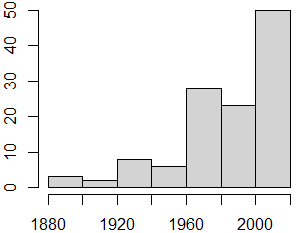
\includegraphics[width=6cm]{letoGradnje_hist.png}
	\caption{Leto gradnje}
	\label{figure:1a}
\end{subfigure}
\begin{subfigure}{0.5\textwidth}
	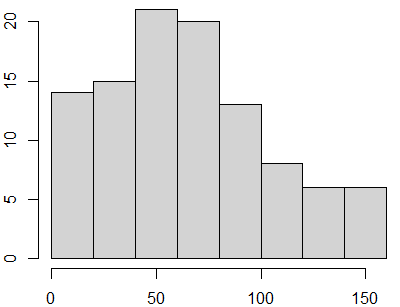
\includegraphics[width=6cm]{povrsina_hist.png}
	\caption{Povrsina}
	\label{figure:1b}
\end{subfigure}

\begin{subfigure}{0.5\textwidth}
	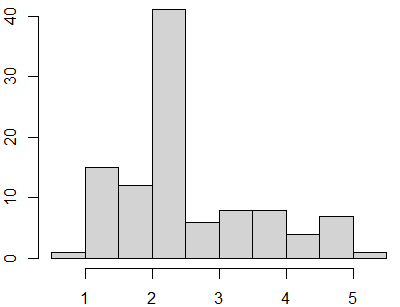
\includegraphics[width=6cm]{oddaljenost_hist.png}
	\caption{Oddaljenost}
	\label{figure:1c}
\end{subfigure}
\begin{subfigure}{0.5\textwidth}
	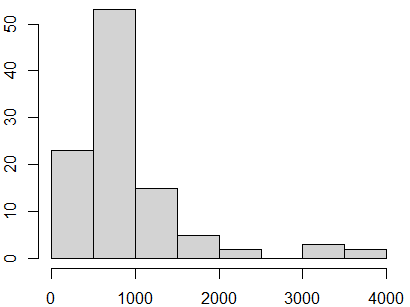
\includegraphics[width=6cm]{skCena_hist.png}
	\caption{Skupna cena}
	\label{figure:1d}
\end{subfigure}
\caption{Histogrami zveznih spremenljivk}
\label{figure:1}
\end{figure}

Spremenljivka $ parkirisce $ pa je diskretna, zato jo lahko predstavimo z
vzorčnim deležem:

\begin{center}
\begin{tabular}{ c|cc }
	& da & ne \\
	\hline
	parkirisce & 0,544 & 0,456 \\
\end{tabular}
\end{center}


\section{Večkratna regresija}

Linearna regresija je analiza, pri kateri ugotavljamo funkcijsko zvezo med
dvema spremenljivkama ($ X $ in $ Y $), pri večkratni regresiji pa funkcijsko
zvezo med več spremenljivkami, kjer je ena odvisna ($ Y $), ostale pa neodvisne.
Cilj analize je najti linearno funkcijo, ki najbolje opiše obnašanje odvisne
spremenljivke v odvisnosti od ostalih spremenljivk. Pri tem pa mora veljati
nekaj predpostavk regresijskega modela:
\begin{enumerate}
	\item $ Y $ je lienarna funkcija neodvisnih spremenljivk $ X_{1}, X_{2}, \dots $
	\item Napake $ \epsilon_{i} $ so med sabo neodvisne,
	\item Napake $ \epsilon_{i} $ imajo konstantno varianco,
	\item Napake $ \epsilon_{i} $ so normalno porazdeljene.
\end{enumerate}

\subsection{Koeficienti korelacije}

Pri modelu večkratne regresije je najprej potrebno preveriti, kako so
neodvisne spremenljivke povezane med sabo. Če so povezane preveč, lahko z neko
spremenljivko opišemo drugo, in tako iz druge ne izvemo nič novega ali pa zelo
malo o odvisni spremenljivki. Korelacijski koeficient med dvema spremenljivkama
lahko izračunamo po naslednji formuli:
\begin{equation}
	\rho\left(X,Y\right) = \frac{Cov\left(X,Y\right)}{\sigma_{X}\sigma_{Y}} =
	\frac{E\left(\left(X-E\left(X\right)\right)\left(Y-E\left(Y\right)\right)\right)}{\sigma_{X}\sigma_{Y}}
\end{equation}
Koeficient korelacije ima vrednost med $ -1 $ in $ 1 $. Če ima vrednost blizu
$ 1 $, sta spremenljivki pozitivno povezani, če pa ima vrednost blizu $ -1 $,
sta negativno povezani. Če vrednost znaša okoli $ 0 $, spremenljivki nista
povezani.
\newline
V spodnji tabeli so predstavljeni korelacijski koeficienti za zvezne
spremenljivke:
\begin{center}
\begin{tabular}{ c|cccc }
	& letoGradnje & povrsina & oddaljenost & skCena \\
	\hline
	letoGradnje & 1.000 & 0.035 & 0.252 & 0.168 \\
	povrsina & 0.035 & 1.000 & -0.058 & 0.829 \\
	oddaljenost & 0.252 & -0.058 & 1.000 & -0.100 \\
	skCena & 0.168 & 0.829 & -0.100 & 1.000 \\
\end{tabular}
\end{center}

Neodvisne spremenljivke $ letoGradnje $, $ povrsina $ in
$ oddaljenost $ imajo medsebojne koeficiente skoraj $ 0 $ z izjemo
$ letoGradnje $ in $ oddaljenost $, ki imata pozitiven koeficient
$ 0.252 $. Spremenljivki sta pozitivno povezani, kar pomeni, da se novejša
stanovanja nahajajo malo bolj izven središča Ljubljane. Vidimo lahko tudi, da
sta spremenljivki $ povrsina $ in $ skCena $ povezani s koeficientom $ 0,829 $,
iz česar lahko sklepamo, da je najemnina stanovanja v Ljubljani odvisna
predvsem od površine le tega.

\begin{figure}[H]
	\centering
	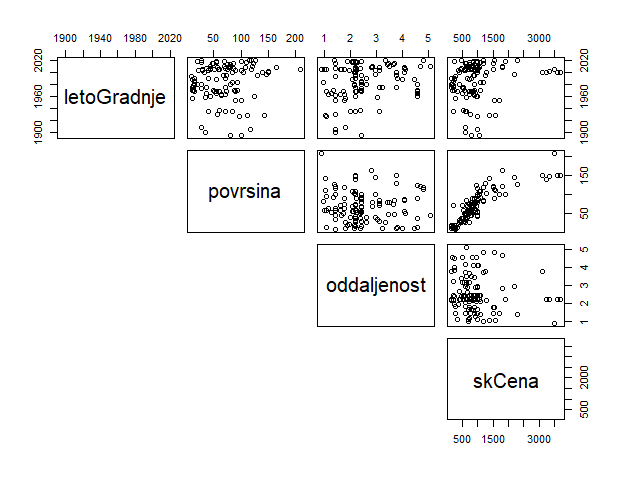
\includegraphics[width=13cm]{pairs.png}
	\caption{Grafični prikaz korelranosti spremenljivk}
	\label{figure:2}
\end{figure}

Iz slike \ref{figure:2} vidimo, kako so podatki 

\subsection{Večkratna regresija}

Neodvinsne spremenljivke našega modeal so $ letoGradnje $, $ povrsina $,
$ oddaljenost $, $ parkirisce $. Odvisna spremenljivka je
$ skCena $. Funkcija bo izgledala tako:
\begin{equation}
	skCena = a+b*letoGradnje+c*povrsina+d*oddaljenost+e*parkirisce+\epsilon
\end{equation}

$ b, c, d $ in $ e $ so koeficienti posameznih neodvisnih spremenljivk. $ a $
predstavlja začetno vrednost, sam po sebi pa nima smisla (stanovanje z $ 0 $ v
pri vseh neodvisnih spremenljivkah bi imelo $ a $ mesečne najemnine, tako
stanovanje pa ne obstaja). $ \epsilon $ predstavlja naključno napako.

Večkratno regresijo sem določil z ukazom \\
{\sf lm(skCena$\sim$letoGradnje+povrsina+oddaljenost+parkirisce, data=data)}. \\
Dobil sem naslednje podatke:
\begin{lstlisting}[language=R,basicstyle=\small]
Call:
lm(formula = skCena ~ letoGradnje + povrsina + oddaljenost +
    parkirisce, data = data)

Residuals:
    Min      1Q  Median      3Q     Max
-765.48 -203.91   -9.88  159.84 1283.37

Coefficients:
             Estimate Std. Error t value Pr(>|t|)
(Intercept) -8806.067   2660.228  -3.310  0.00131 **
letoGradnje     4.499      1.353   3.325  0.00124 **
povrsina       15.714      1.020  15.410  < 2e-16 ***
oddaljenost   -60.497     38.036  -1.591  0.11494
parkirisce   -184.771     79.226  -2.332  0.02174 *
---
Signif. codes: 0 '***' 0.001 '**' 0.01 '*' 0.05 '.' 0.1 ' ' 1

Residual standard error: 371.6 on 98 degrees of freedom
Multiple R-squared:  0.7293, Adjusted R-squared: 0.7183
F-statistic: 66.01 on 4 and 98 DF, p-value: < 2.2e-16
\end{lstlisting}

Iz tabele koeficientov (Coefficients) lahko razberemo koeficiente naše
funkcije, skupaj z njihovo napako ocene, t statistiko in p vrednostjo. P
verjetnost nam pomaga pri zavračanju ničelne hipoteze modela: vrednosti
koeficientov so enake $ 0 $. Pri vseh spremenljivkah razen $ oddaljenost $ so
p vrednosti manjše od $ 0.05 $, zato za te spremenljivke ničelno hipotezo
zavrnemo. Koeficienti spremenljivk $ letoGradnje, povrsina $ in $ parkirisce $
so po vrsti $ 4.499, 15.714 $ in $ -183.771 $. Ker ničelne hipoteze pri
spremenljivki $ oddaljenost $ ne zavrnemo, ta za naš model ni pomembna. Naša
funkcija je tako naslednja:
\begin{equation}
	skCena = -8806.067+4.499*letoGradnje \newline +15.714*povrsina-183.771*parkirisce+\epsilon
\end{equation}

\subsection{Preverjanje ustreznosti modela}

Prirejeni $ R^{2} $ (Adjusted R-squared) nam pove, kako veliko nam o
spremenljivki $ skCena $ pove naš model. Vrednost $ 0.7183 $ nam pove, da naš
regresijski model pojasni $ 71.83\% $ sprememb spremenljivke $ skCena $. Ker pa
je standardni odklon naključnih napak (Residual standard error) precej velik
($ 371.6 $), lahko sklepamo, da model ni najboljši. Zato preverimo še štiri
predpostavke o regresijskem modelu. Te lahko preverimo z štirimi diagnostičnimi
grafi:
\begin{figure}[H]
	\centering
	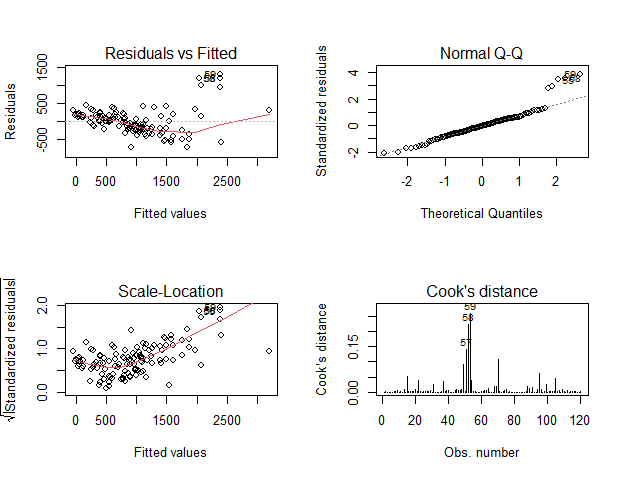
\includegraphics[width=13cm]{diagnosticGraphs.png}
	\caption{Diagnostični grafi}
\end{figure}

Zgornji levi graf (Residuals vs Fitted) preverja linearnost modela. Prikazuje
ostanke $ \epsilon_{i} $ v odvisnosti od predvidenih vrednosti. Točke
oblikujejo negativno linearno funkcijo, kar pomeni, da v našem modelu manjka
linearna funkcija neke neznane spremenljivke. Naš model zato ni dober in bi se
ga dalo izboljšati.

Zgornji desni graf (Normal Q-Q) prikazuje normalnost porazdelitve
standardiziranih ostankov. Če točke tvorijo premico, lahko sklepamo, da so
napake normalno porazdeljene. Ker točke na desni strani odstopajo od premice,
napake ne izgledajo normalno porazdeljene. To dodatno potrdi rezultat ukaza
{\sf shapiro.test(fit\$residuals)}, ki hipotezo o normalnosti ovrže s p
vrednostjo $ 1.102e-05 $.

Spodnji levi graf (Scale-Location) predstavlja varianco napak, ki naj bi bile
konstantne. Na grafu se variance zelo razlikujejo, to pa potrjuje tudi ukaz
{\sf ncvTest(fit)}, ki hipotezo o konstantni varianci ovrže s p vrednostjo
$ < 2.22e-16 $.

Spodnji desni graf (Cook's distance) prikazuje, kateri podatki najbolj
odstopajo od modela. Pri tem nas zanima, kako vplivajo na model. Točke s
preveliko razdaljo dobimo z ukazom {\sf points $\leftarrow$ which(cooks.distance(fit) $ > $ 4/101)}.
Njihov vpliv preverimo z ukazom {\sf any(cooks.distance(fit)[points]$ > $=qf(0.5, 4, 98))}.
Ker vrne False, to pomeni, da nobena točka ne vpliva preveč na model in jih
zato ni potrebno odstraniti.

Za naše koeficiente pa lahko tudi izračunamo intervale zaupanja za $ 95\% $
gotovost. Intervale za vsak koeficient dobimo z ukazom {\sf confint(fit)}, ki
nam vrne naslednjo tabelo:
\begin{center}
\begin{tabular}{ c|cc }
	& 2.5\% & 97.5\% \\
	\hline
	(Intercept) & -14085.203 & -3526.931 \\
	letoGradnje & 1.814 & 7.184 \\
	povrsina & 13.691 & 17.738 \\
	oddaljenost & -135.979 & 14.984 \\
	parkirisce & -341.992 & -27.551 \\
\end{tabular}
\end{center}
Intervali zaupanja so za vse koeficiente precej veliki, zato naš model ni
ustrezen.

\section{Zaključek}

Večkratnemu regresijskemu modelu manjka neka neznana linearna spremenljivka.

\section{Literatura}

[0]
https://www.distance.to/

[1] Analiza dejavnikov oglaševanih cen rabljenih stanovanj v Ljubljani in njeni
okolici, Sonja Friškovec, Aleksander Janeš, Univerza na Primorskem, jesen 2010

[2] Dejavniki oblikovanja prodajnih cen stanovanj, Mojca Repič, Ljubljana,
oktober 2014

[3] \href{https://www.researchgate.net/publication/239329925_A_New_Test_of_Symmetry_about_an_Unknown_Median}
enačba 11

[4] \href{https://gitlab.com/ul-fri/ovs/projekt/-/blob/master/regresija.pdf}{A}

\end{document}